% 第12章第3节：由树分解构建动态规划（包含局部作用域的袋、接口的分隔性质、从叶袋得到消元序）。

\section{由树分解构建动态规划}
\label{sec:graph-dp-from-decomposition}

上一节从消元次序出发得到树分解。本节反过来，从一个给定的树分解出发，直接规定局部子问题。需要证明的有两件事：每个局部项都能整体放进某个袋，这样它才有处可放；相邻两袋的接口确实把两侧的变量隔开，这样以接口为索引的摘要才足够。最后从叶袋向内处理变量，读出一个与分解相容的消元次序，说明树分解既能作为构建的输入，也能作为消元结果的显式表示。

\subsection{包含局部作用域的袋}
\label{sec:graph-dp-clique-containment}

计算时每个局部函数要整个放进一个袋，因为袋表需要同时索引它的全部变量。一个作用域$S_a$在原始图上是团：其中任意两个变量同在$\phi_a$中，因而相邻。但树分解的定义只要求每条边被某个袋覆盖，三个变量两两成边时，三条边似乎可能分别落在三个不同的袋中。下面先证明一个关于子树的一般事实，再由它推出这种情况不会发生。

把每个顶点$v$的出现位置$T_v$看成袋树中的一棵连通子树。若$u,v$相邻，边覆盖给出一个同时含$u,v$的袋，于是$T_u$与$T_v$相交。对一个团$C$，各$T_v$（$v\in C$）两两相交；要证明的是它们有一个公共节点。

\begin{lemma}[两两相交的子树有公共节点]
\label{lem:graph-dp-subtree-helly}
设$\mathcal T$是有限树，$T_1,\ldots,T_k$（$k\geq1$）是它的非空连通子树，并且两两相交。则存在节点同时属于全部$T_j$。
\end{lemma}

\begin{proof}
任取$\mathcal T$的一个节点作为根。与引理~\ref{lem:graph-dp-unique-internal}的证明相同，每个$T_j$有唯一一个离根最近的节点，记为$r_j$，并且$T_j$的每个节点都是$r_j$的后代（含$r_j$本身）。取$j^\ast$使$r_{j^\ast}$的深度在$r_1,\ldots,r_k$中最大，下面证明$r_{j^\ast}$属于每个$T_l$。

$l=j^\ast$时结论由定义成立。$l\neq j^\ast$时，$T_l\cap T_{j^\ast}$中有某个节点$x$；$x\in T_{j^\ast}$，因而$x$是$r_{j^\ast}$的后代。

考察$T_l$中从$x$到$r_l$的路径，它留在$T_l$中。若$r_l$不是$r_{j^\ast}$的后代，这条路径从$r_{j^\ast}$下方的子树走到外部，必须经过$r_{j^\ast}$，因为这棵子树与外部只通过$r_{j^\ast}$与其父节点之间的边相连；于是$r_{j^\ast}\in T_l$。若$r_l$是$r_{j^\ast}$的后代，则$r_l$的深度不小于$r_{j^\ast}$的深度；而按$j^\ast$的选取，$r_l$的深度又不大于$r_{j^\ast}$的深度，所以$r_l=r_{j^\ast}$，同样有$r_{j^\ast}\in T_l$。
\end{proof}

\begin{lemma}[团被某个袋容纳]
\label{lem:graph-dp-clique-in-bag}
设$(\mathcal T,\{B_t\}_{t\in T})$是$\mathcal G$的树分解，$C\subseteq V$是$\mathcal G$中的非空团，则存在节点$t\in T$使$C\subseteq B_t$。
\end{lemma}

\begin{proof}
由顶点覆盖与运行交集，每个$T_v$（$v\in C$）是非空连通子树。$C$中任意两个顶点$u,v$相邻，由边覆盖，$T_u\cap T_v\neq\varnothing$。由引理~\ref{lem:graph-dp-subtree-helly}，存在节点$t$属于全部$T_v$，即$C\subseteq B_t$。
\end{proof}

图~\ref{fig:graph-dp-clique-in-bag}画出了证明中的几棵子树：每个变量的出现位置向上延伸到自己的最高节点，最高节点最深的那个变量，它的最高节点被其余各子树“经过”，因而就是要找的袋。

\begin{figure}[!htb]
  \centering
  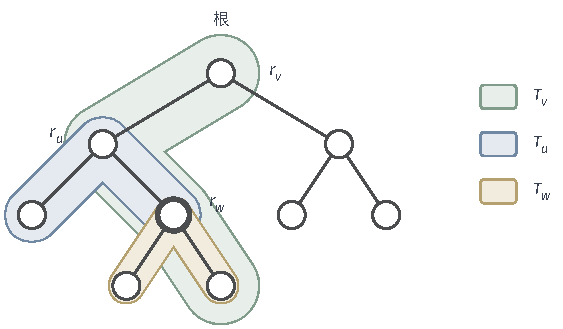
\includegraphics[width=102.648mm]{figures/01-basic-mathematics/04-graphs/tikz/c5-clique-in-bag/figure.pdf}
  \caption{团$\{u,v,w\}$被某个袋容纳的论证。袋树以顶部节点为根，三种颜色的区域分别是$T_u$、$T_v$、$T_w$，标签$r_u,r_v,r_w$标出各自离根最近的节点。$r_w$最深；$T_u$、$T_v$都要与$T_w$相交，而它们的最高节点不比$r_w$深，所以必须经过$r_w$。粗圈节点$r_w$的袋同时含$u,v,w$。}
  \label{fig:graph-dp-clique-in-bag}
\end{figure}

由引理~\ref{lem:graph-dp-clique-in-bag}，原始图的任一树分解中，每个局部函数的完整作用域都被某个袋整体容纳。因此在原始图上构造树分解就足够了，不需要额外记录高阶作用域；第~\ref{sec:graph-local-functions}节所说的“结构以原始图为依据、计算保留完整函数”在这里得到保证。

要找出容纳$S_a$的袋，只需在$T_v$（$v\in S_a$）中最小的一个里逐个检查袋是否包含$S_a$。同样，第~\ref{sec:graph-dp-query-structure}小节补成团的保留集$R$也一定被某个袋容纳。

\paragraph{树宽的下界}
引理~\ref{lem:graph-dp-subtree-helly}也给出第~\ref{sec:graph-tree-decomposition}小节几个例子的下界。一条边要求某个袋含两个顶点，所以含边的图宽度不能小于$1$；至少含一条边的树因而树宽恰为$1$。

四个顶点的环$1-2-3-4-1$没有宽度为$1$的树分解。给任一树分解选根，取环上的顶点$w$使$T_w$的最高节点最深。$w$在环上的两个邻居$u,v$各自与$w$相邻，于是$T_u$、$T_v$都与$T_w$相交；引理证明中的论证表明，$T_w$的最高节点同时属于$T_u$与$T_v$。这个袋含$u,v,w$三个顶点，所以宽度至少为$2$，四环的树宽恰为$2$。

这一论证对任何环都适用：含环的图树宽至少为$2$。因此树宽为$1$的图恰好是至少含一条边的森林。森林的各个分量分别按树的方法分解，再用任意的边把各分量的袋树连成一棵树；不同分量没有公共顶点，这些连接不影响运行交集。图~\ref{fig:graph-dp-ladder-decomposition}的梯子含环，又有宽度为$2$的分解，所以树宽恰为$2$；按同样的方式扫描，任意长的梯子树宽都是$2$。

四个顶点两两相邻的完全图恰好相反。整个顶点集是一个团，由引理~\ref{lem:graph-dp-clique-in-bag}，任何树分解都有一个袋装下全部四个顶点，宽度至少为$3$，所以树宽为$3$。同样，$n$个顶点的完全图树宽为$n-1$，树分解对它没有任何节省。

可见树宽衡量的是图与树的接近程度：一条边需要两个变量同时出现，一个环迫使某处至少三个变量同时出现，而一个大团迫使它的全部变量同时出现。

\subsection{接口的分隔性质}
\label{sec:graph-dp-interface-separation}

树上消息的正确性依赖于一件事：删去一条边后，两侧除了接收变量以外没有共同的变量。袋树上，这件事由运行交集保证。删去袋树边$\{s,t\}$后，袋树分成两部分；记$s$一侧全部袋中出现的变量为$V_{s|t}$，$t$一侧为$V_{t|s}$，接口为$B_s\cap B_t$。

若某个变量$v$在两侧都出现，从它在$s$侧的某个出现位置到$t$侧的某个出现位置，袋树路径必须经过边$\{s,t\}$；由运行交集，$B_s$与$B_t$都含$v$。所以
\begin{equation}
V_{s|t}\cap V_{t|s}\subseteq B_s\cap B_t,
\label{eq:graph-dp-interface-separation}
\end{equation}
即接口把两侧的变量隔开：固定接口取值后，两侧的其余变量互不重叠。

只有变量不重叠还不够，还要确认两侧没有被某个局部项直接连在一起，否则两侧的其余变量仍不能分别优化。下面的引理说明，每个局部项都整体落在某一侧。

\begin{lemma}[接口分隔两侧]
\label{lem:graph-dp-interface-separation}
设$(\mathcal T,\{B_t\}_{t\in T})$是原始图的树分解，$\{s,t\}$是袋树的边。则式~\eqref{eq:graph-dp-interface-separation}成立；并且对每个局部函数$\phi_a$，$S_a\subseteq V_{s|t}$或$S_a\subseteq V_{t|s}$。因此，任何局部项都不同时读取$V_{s|t}\setminus B_t$中的变量与$V_{t|s}\setminus B_s$中的变量。
\end{lemma}

\begin{proof}
式~\eqref{eq:graph-dp-interface-separation}已在上面证明。由引理~\ref{lem:graph-dp-clique-in-bag}，$S_a$被某个袋$B_x$容纳，$x$在$s$一侧或$t$一侧，于是$S_a\subseteq V_{s|t}$或$S_a\subseteq V_{t|s}$。若某个$\phi_a$同时读取$y\in V_{s|t}\setminus B_t$与$z\in V_{t|s}\setminus B_s$，不妨设$S_a\subseteq V_{s|t}$，则$z\in V_{s|t}\cap V_{t|s}\subseteq B_s$，与$z\notin B_s$矛盾；另一种情形同理。
\end{proof}

在选了根的袋树中，取$t=p(u)$。$u$下方各袋（含$u$本身）中出现而不在接口$S_u$中的变量，由式~\eqref{eq:graph-dp-interface-separation}不会出现在其余袋中，它们正是$u$下方各节点的内部变量之并。引理~\ref{lem:graph-dp-interface-separation}说明，固定$\bm x_{S_u}$后，这些变量与其余变量之间没有遗漏的直接耦合，所以$u$下方可以单独摘要成一张以$\bm x_{S_u}$为索引的表。这正是第~\ref{sec:graph-dp-construction-goal}小节的第二项要求；第~\ref{sec:graph-dp-min-cost-correctness}小节用它证明数值递推的正确性。

\subsection{从叶袋得到消元序}
\label{sec:graph-dp-decomposition-to-order}

给定一个宽度为$w$的树分解，可以反过来读出一个诱导宽度不超过$w$的消元次序。思路是从叶袋开始：叶袋中不在父袋里的变量只出现在这个叶袋中，消去它们时，它们的邻居都在叶袋里，产生的填充边也都落在叶袋里。

\paragraph{算法}
输入是图$\mathcal G$的一个树分解，选定一个根；输出是全部顶点的一个消元次序。维护当前图（初值为$\mathcal G$）、当前袋树（初值为输入分解）和已输出的次序（初值为空）。当前袋树不只一个节点时，反复处理一个非根叶节点$\ell$，记其父节点为$p$：
\begin{itemize}
  \item 若$B_\ell\subseteq B_p$，直接从袋树中删去$\ell$；
  \item 否则按任意次序依次消去$B_\ell\setminus B_p$中的变量：把每个变量追加到次序末尾，在当前图中把它的邻居补成团并删去它，同时把它从$B_\ell$中删去；此时$B_\ell\subseteq B_p$，再删去$\ell$。
\end{itemize}
最后只剩根袋，按任意次序消去其中剩余的变量。

\begin{algorithm}[由树分解读出消元次序]
\label{alg:graph-dp-decomposition-to-order}
输入：有限无向图$\mathcal G$的树分解，以及选定的根。输出：$\mathcal G$的一个消元次序。
\begin{enumerate}
  \item 令当前图为$\mathcal G$的副本，当前袋树为输入的分解，次序为空。
  \item 若当前袋树只剩根，转第4步。否则取一个非根叶节点$\ell$及其父节点$p$。
  \item 依次消去$B_\ell\setminus B_p$中的变量（追加到次序、补团、从当前图和$B_\ell$中删去），然后删去节点$\ell$，回到第2步。
  \item 按任意次序消去根袋中剩余的变量，输出次序。
\end{enumerate}
\end{algorithm}

\paragraph{正确性}
算法维持一个不变量：当前袋树（各袋只保留尚未消去的变量）是当前图的树分解。开始时它就是输入分解。

设叶节点$\ell$中有变量$v\notin B_p$。由运行交集，$T_v$连通，而$\ell$在袋树中只与$p$相邻、$p\notin T_v$，所以$T_v=\{\ell\}$：$v$只出现在$B_\ell$中。由边覆盖，$v$在当前图中的每条边都被某个含$v$的袋覆盖，只能是$B_\ell$，所以$v$的当前邻居全在$B_\ell$中，个数至多$|B_\ell|-1\leq w$。消去$v$补入的填充边两端都在$B_\ell$中，被$B_\ell$覆盖；从$B_\ell$中删去$v$后，三个条件对新的当前图仍然成立。

$B_\ell\subseteq B_p$时删去$\ell$也保持不变量：$\ell$覆盖的顶点和边都被$B_p$覆盖；含某个变量的节点集合去掉一个叶节点后仍然连通。最后剩下根袋时，当前图的全部顶点都在根袋中，每个顶点的当前邻居至多$|B_r|-1\leq w$个。

所以每个顶点被消去时，剩余邻居数都不超过$w$，得到的消元次序诱导宽度不超过分解的宽度。

\paragraph{执行过程}
以图~\ref{fig:graph-dp-ladder-decomposition}的梯子为例，以$\{3,5,6\}$为根，逐步处理叶袋：
\begin{itemize}
  \item 叶袋$\{1,2,4\}$的父袋是$\{2,4,5\}$，消去$1$：它的当前邻居为$\{2,4\}$，补入$\{2,4\}$；剩余的$\{2,4\}$包含于父袋，删去该叶。
  \item 接着$\{2,4,5\}$成为叶，消去$4$：当前邻居为$\{2,5\}$，已相邻。
  \item 再处理$\{2,3,5\}$，消去$2$：当前邻居为$\{3,5\}$，补入$\{3,5\}$。
  \item 最后在根袋中依次消去$3,5,6$。
\end{itemize}

得到的次序为$(1,4,2,3,5,6)$，各步剩余邻居数依次为$2,2,2,2,1,0$，诱导宽度为$2$，等于分解的宽度。每一步补入的填充边都落在当时的叶袋里，正如正确性论证所说。
